\section{Introduction}

Evolutionary biology has made great strides in understanding both the genetics of ecological adaptation \cite{hoekstra2006single, schluter2009genetics, arnegard2014genetics} and how the speciation process unfolds \cite{coyne2004speciatjon, gavrilets2004fitness, noor2006speciation, seehausen2014genomics}, but we are just beginning to understand how natural selection and gene flow interact in affecting genomic divergence between emerging species that adapt to different ecological regimes in the face of gene flow \cite{feder2012genomics}, or indeed if they do \cite{bierne2013pervasive}. The advent of high-throughput sequencing technology offers the opportunity to examine the genomic signatures of selection and gene flow in speciation. However, disentangling the various processes affecting genomic differentiation is a nontrivial problem \cite{charlesworth1998measures, noor2009islands, cruickshank2014reanalysis}.

One popular conceptual model \cite{wu2001genic} suggests that genomic divergence at the onset of speciation without geographical isolation will be concentrated in ‘islands’ carrying the genes underlying those traits that are responsible for functional divergence between the emerging species. These islands are thought to persist in the face of gene flow due to the effects of divergent or disruptive natural selection. Later in the process, as gene flow between incipient species is further reduced, these islands would gradually increase in size until most of the genome becomes reproductively isolated.

The Wu \cite{wu2001genic} model and its descendants \cite{wu2004genes, via2008genetic, feder2012genomics} have been tested in genome scans of several young species pairs with mixed support \cite{turner2005genomic, ellegren2012genomic, gagnaire2013genetic, martin2013genomewide, renaut2013genomic, ruegg2014role}, but not all of these species pairs exhibit strong ecological and phenotypic divergence \cite{harr2006genomic, carneiro2010speciation}. However, because the Wu model is explicitly framed in the context of ecological and functional divergence, we suggest its utility should ideally be tested in replicate species pairs with distinct phenotypic and putatively adaptive divergence of similar magnitude but different ages.

The Wu model suggests several key predictions when comparing ecological divergence on differing timescales in sympatric species. In younger pairs where gene flow remains possible, we expect to see little genomewide divergence. However, a relatively small number of outlier regions associated with traits under selection may experience strongly elevated divergence relative to the rest of the genome. In older ecologically divergent pairs that no longer experience gene flow, we expect increased genomewide divergence. This increased divergence due to reproductive isolation will make it more difficult to detect outlier regions associated with specific traits. In cases where ecological divergence has occurred in parallel between young and old pairs, it will be considerably easier to detect similar outlier regions when comparing young pairs, as the growing genomic divergence due to reproductive isolation will hide regions associated with phenotypic differences between species.

Here, we utilize whole-genome resequencing to examine ecologically divergent species within three separate radiations of haplochromine cichlids, ranging in age from several ten thousand to several millions of years \cite{genner2007age}. African cichlid fish are a model system for the study of adaptive radiation and speciation \cite{fryer1972cichlid, seehausen2006african, seehausen2015process}. Cichlids are one of the most ecologically diverse and species-rich groups of fishes, and their rapid radiations within the lakes of Eastern Africa are some of the most impressive examples of rapid vertebrate evolution on the planet. The large species richness and ecological diversity of haplochromine cichlids that has evolved in many replicate adaptive radiations in different African lakes enable us to select sympatric species pairs with similar eco-phenotypic divergence (similar `ecomorphs' sensu Williams 1972 \cite{williams1972origin}) at nearly any stage of speciation and post-speciational divergence during adaptive radiation, maximizing the utility of whole-genome comparisons.

We focus here on a consistent pattern of ecological and phenotypic divergence between haplochromine cichlids from the two relatively young sympatric radiations of Victoria and Kivu, as well as an older radiation, possibly of partially allopatric origin in Lake Mweru. Lake Victoria contains an extremely young and highly diverse cichlid radiation that originated between 10,000 and 100,000 years ago \cite{seehausen2002patterns, genner2007age, salzburger2014ecology}. Nearby Lake Kivu hosts a slightly older radiation, between 100,000 and 250,000 years in age \cite{genner2007age, bezault2011population, salzburger2014ecology}. Current evidence suggests that cichlids in these radiations evolved into a diverse array of ecomorphs within each lake, many of which are replicated between the lakes. Our final example, Lake Mweru in the upper Congo (Zambia/DRC), hosts several different lineages of haplochromine cichlids that probably began to evolve their ecological specializations prior to invading the lake. The age of the most recent common ancestor for the Mweru lineages is nearly as old as the age of the entire haplochromine tribe, between 4 and 23 million years ago \cite{genner2007age, wagner2012ecological, friedman2013molecular} (Figure \ref{UL_fig1}).

\begin{figure}
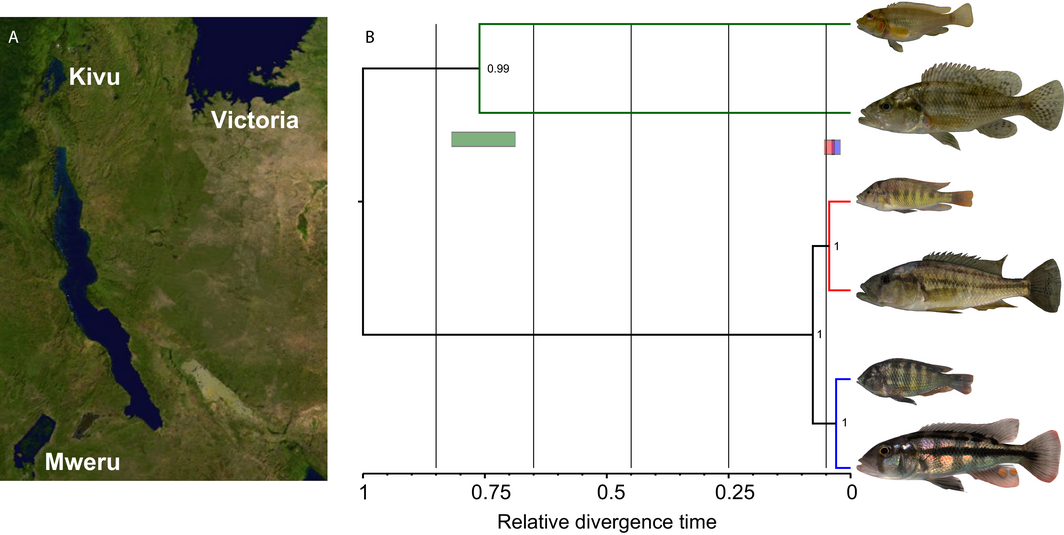
\includegraphics[width=\textwidth]{uLakes/figures/fig1}
\caption{The study system. \textbf{A.} Locations of the three lakes in our study: Victoria (Tanzania/Uganda/Kenya), Kivu (DRC/Rwanda) and Mweru (Zambia/DRC). \textbf{B.} Whole mitogenome tree of the six species in this study. From top: Orthochromis `red cheek' (Mweru), Serranochromis `checkerboard' (Mweru), {\em Paralabidochromis paucidens} (Kivu), {\em Harpagochromis vittatus} (Kivu), {\em Paralabidochromis flavus} (Victoria) and {\em Harpagochromis} `checkmate' (Victoria), three evolutionary replicates of pairs of archetypal cichlid ecomorphs. Fish images indicate the approximate adult body size of each species relative to the others. Numbers at the nodes indicate posterior probabilities. Shaded bars adjacent to the x-axis indicate the 95\% HPD of relative divergence times for each insectivore-piscivore comparison.}
\label{UL_fig1}
\end{figure}

Against these different speciation contexts, we have identified in each lake a pair of sympatric species that exhibit ecologies and phenotypes that are very different from each other and very similar between lakes despite differences in the time to most recent common ancestor of each lake pair, representing two archetypal lake cichlid ecomorphs. In each lake, we compare a large suction feeding fish-eating species that is a habitat generalist to a small biting insect-eating species, living strictly on rocky reefs. This comparison involves divergence in body size, trophic level, feeding mode, habitat, social behaviour (i.e. territoriality) and male coloration and represents a major axis of ecological diversity within each radiation. In Lake Victoria, we compare the fish-eating {\em Harpagochromis} sp. `checkmate' to the insect-eating {\em Paralabidochromis flavus} \cite{seehausen1998mbipi}. In Kivu, we compare {\em Harpagochromis vittatus} to {\em Paralabidochromis paucidens} \cite{snoeks1994haplochromines}. These species, despite being from different lakes, were originally assigned to the same genera on the basis of highly similar morphology \cite{greenwood1979towards}, although current molecular evidence strongly rejects across-lake monophyly of {\em Harpagochromis} and {\em Paralabidochromis} \cite{bezault2011population}. From Lake Mweru, we sequenced the fish-eating species {\em Serranochromis} sp. `checkerboard' and the small insect picker, {\em Orthochromis} sp. `red cheek,' each from a different ancient haplochromine lineage that coexist in sympatry in Lake Mweru.

Hybridization between cichlid species of the Lake Victoria radiation generates viable and fertile offspring, suggesting that strong intrinsic isolation has not yet evolved between species in the radiation \cite{stelkens2009genetic, stelkens2015hybrid}. Lake Kivu species have rarely been maintained in aquaria, but evidence from other haplochromines suggests that crosses between species in its age range are generally viable. However, {\em Serranochromis}  and {\em Orthochromis} diverged from each other, as well as from East African haplochromines like those of Victoria, at least 4-9 million years ago \cite{genner2007age, friedman2013molecular} and possibly more than 20 million years ago \cite{genner2007age, wagner2012ecological, schwarzer2012repeated} and hybridization studies suggest that crosses at this level of phylogenetic distance in haplochromine cichlids generally exhibit complete intrinsic postzygotic reproductive isolation \cite{stelkens2009genetic, stelkens2015hybrid}.

To examine the genomic signature of ecological and reproductive divergence in these three species pairs from three different lakes, we sequenced the whole genome of one individual of each species. We examine overall levels of nuclear and mitochondrial divergence, establish that the three sympatric species pairs are reciprocally monophyletic and then investigate patterns of relative and absolute divergence in outlier loci and in the rest of the genome. By studying three pairs of archetypal cichlid radiation phenotypes (`ecomorphs'), we also assess whether there is a detectable genomic signal of parallel divergent evolution associated with the origin of convergent phenotypes across the three radiations, and how this signature is affected by comparisons of different ages and evolutionary histories.
